\documentclass[DIV=calc, paper=a4, fontsize=11pt]{scrartcl}


\usepackage{makeidx}
\usepackage{graphicx}
\usepackage{flushend}

\usepackage{lmodern}
\usepackage[left=1.5cm,right=1.5cm,top=2.5cm,bottom=2cm]{geometry}
\usepackage{float}		
\bibliographystyle{plain} 
\pagestyle{plain} 
\pagenumbering{arabic}
\usepackage{fancyhdr} 	


\usepackage[T1]{fontenc}
\usepackage[utf8]{inputenc}
\usepackage[spanish]{babel}
\usepackage{hyperref}
\usepackage{graphicx}

\usepackage{lipsum}
\usepackage[protrusion=true,expansion=true]{microtype}
\usepackage{amsmath,amsfonts,amsthm}
\usepackage[svgnames]{xcolor}
\usepackage[svgnames]{xcolor}
\usepackage{booktabs}
\usepackage{fix-cm}
\usepackage{multicol}
\usepackage{siunitx}
\newenvironment{Figura}
  {\par\medskip\noindent\minipage{\linewidth}}
  {\endminipage\par\medskip}

\usepackage{sectsty}
\allsectionsfont{\usefont{OT1}{phv}{b}{n}}

\usepackage{fancyhdr}
\pagestyle{fancy}
\usepackage{lastpage}

\lhead{}
\chead{}
\rhead{}

\lfoot{}
\cfoot{}
\rfoot{\footnotesize Page \thepage\ of \pageref{LastPage}}

\renewcommand{\headrulewidth}{0.0pt}
\renewcommand{\footrulewidth}{0.4pt}

\usepackage{lettrine}
\newcommand{\initial}[1]{\lettrine[lines=3,lhang=0.3,nindent=0em]{
\color{DarkGoldenrod}{\textsf{#1}}}{}}

\usepackage{titling}

\newcommand{\HorRule}{\color{DarkGoldenrod} \rule{\linewidth}{1pt}}

\pretitle{\vspace{-120pt} \begin{flushleft} \HorRule \fontsize{22}{35} \usefont{OT1}{phv}{b}{n} \color{DarkRed} \selectfont}

\title{Simulación Electrónica Analógica del Oscilador Armónico\\ %Aquí va el nombre de la práctica 
Práctica 4} %Numero de la práctica 

\posttitle{\par\end{flushleft}\vskip 0.5em}

\preauthor{\begin{flushleft}\large \lineskip 0.5em \usefont{OT1}{phv}{b}{sl} \color{DarkRed}}

\author{García Perez Angel Yair\\
Misael Iván Macías Márquez}

\postauthor{\footnotesize \usefont{OT1}{phv}{m}{sl} \color{Black}

\vspace*{0.1cm} Facultad de Ciencias, UNAM

\par\end{flushleft}\HorRule}

\date{Viernes 8 de Abril de 2022\\Semestre 2022-2}


\begin{document}

\maketitle


\begin{abstract}
\textbf{Resumen:} Se simuló con amplificadores operacionales el sistema mecánico del oscilador armónico sin rozamiento y se efectuaron $3$ simulaciones con diferentes valores de condiciones iniciales, para la primer simulación se usaron las condiciones $X_{0}=0.5 m$, $V_{0}= 2\frac{m}{s}$ para la segunda $X_{0}=0 m$, $V_{0}= -10\frac{m}{s}$ y para la tercera $X_{0}=10 m$, $V_{0}= 0\frac{m}{s}$.
\end{abstract}

\begin{multicols}{2}




\section*{Introducción}

\subsection*{Objetivos}

\begin{enumerate}
    \item Simular con amplificadores operacionales el sistema mecánico del oscilador armónico sin rozamiento .
    
    \item Efectuar 3 simulaciones diferentes de condiciones iniciales, por ejemplo: $V_{0X} = 0$ y $X_0 > 0$, $V_{0X}<0$ y $X_0 =0$, $V_{0x}> 0$ y $X_{0}>0$, etc.
    
    \item Realizar el circuito con representación en el proto-board usando algún software como los mencionados en clase.
\end{enumerate}

\subsection*{Oscilador Armónico Simple}

Se dice que un sistema cualquiera, mecánico, eléctrico, neumático, etc, es un oscilador armónico si, cuando se deja en libertad fuera de su posición de equilibrio, vuelve hacia ella describiendo oscilaciones sinusoidales en torno a dicha posición estable[1].
\\\\
A partir de la segunda ley de Newton $ F=m\frac{d^2 x}{dt^2} $ y la ley de Hooke $F=-kx$ se llega a la ecuación para el Oscilador Armónico Simple[1]:
$$ -kx = m\frac{d^2 x}{dt^2} $$
\begin{equation}
  \iff  m\frac{d^2 x}{dt^2} + kx = 0 %\hspace{1cm} x(0) = X_0 \hspace{0.2cm} x'(0)=0
\end{equation}
La solución de esta ecuación diferencial ordinaria la podemos escribir como[1]:
$$ x= A\sin{(\omega t)}+B\cos{(\omega t)} $$
Donde $A$ y $B$ dependen de las condiciones iniciales y donde:
$$ \omega =\sqrt{\frac{k}{m}} $$
$k$ es la constante del resorte y $m$ la masa del oscilador[1].
%aplicando la transformada de Laplace,

%\begin{equation*}
%    m[s^2 X(s)-sx(0) -x'(0)]+kX(s) = 0
%\end{equation*}

%\begin{equation*}
%    ms^2X(s)-msX_0 +kX(s)=0
%\end{equation*}

%\begin{equation*}
%    X(s) = \frac{mX_0 s}{ms^2 + k} = \frac{X_0 s}{s^2 + \frac{k}{m}}
%\end{equation*}

%\begin{equation*}
%    \therefore \hspace{1cm} x(t) = X_0 \cos{\sqrt{\frac{\omega}{k}}t}
%\end{equation*}

\subsection*{Amplificador inversor}
Para el amplificador inversor se tiene la ecuación[2]:
\begin{equation}
    v_0= -\frac{R_f}{R_i} v_i
\end{equation}

Donde $v_{i}$ es el voltaje de entrada, $v_{0}$ el voltaje de salida, $R_{i}$ la resistencia conectada en serie con la entrada del circuito y $R_{f}$ la resistencia conectada en serie con la entrada del circuito y con la salida del mismo[2].

\subsection*{Amplificador operacional como integrador}


Para el amplificador inversor integrador se tiene la ecuación[3]:
\begin{equation}
    v_0 =- \frac{1}{RC} \int v_i dt + V_C(t_0)
\end{equation}

Donde $v_{i}$ es el voltaje de entrada, $v_{0}$ el voltaje de salida, $R$ la resistencia, $C$ la capacitancia y $V_C$ una constante de integración[3].




\section*{Metodología}

\begin{Figura}
    \centering
    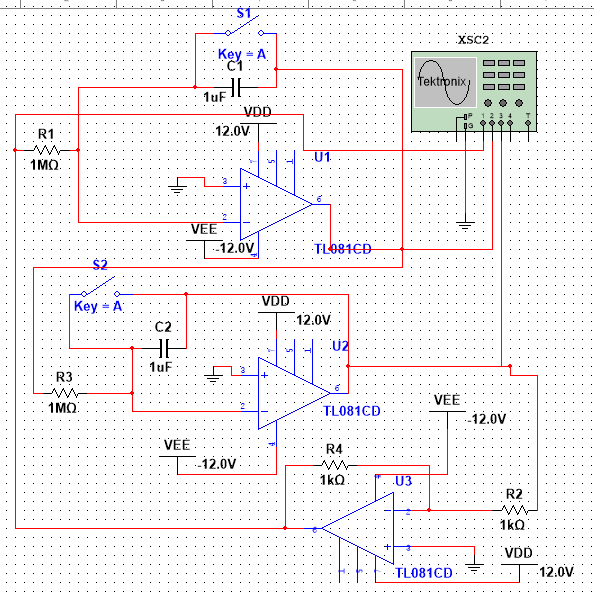
\includegraphics[width=1\textwidth]{Metodologia/Simulacion.png}
    \captionof{figure}{Diagrama del circuito que se usó para simular un oscilador
armónico sin rozamiento.}
    \label{fig}
\end{Figura}

En el simulador Multisim primero se armó un circuito inversor integrador con un amplificador operacional \textbf{TL081}, este se alimentó con una fuente bipolar de $\pm 12V$, también se utilizó un condensador de $1 \mu F$, una resistencia de $1 M \Omega$ y un interruptor. 
\\\\
La salida de este circuito se conecto a la entrada de un segundo circuito inversor integrador, este tenia las mismas características que el primero, la salida del segundo circuito inversor integrador se conecto a la entrada de un amplificador inversor, la salida del amplificador se conecto a la entrada del primer circuito inversor integrador.
\\\\Para el amplificador inversor se utilizó 2 resistencias de $1k\Omega$, una fuente bipolar de $\pm 12V$, un amplificador operacional \textbf{TL081CD} y cables.
\\\\
Para que el sistema mecánico tuviera una condición inicial de velocidad $V_{0}$ simplemente se conecto una fuente de poder en el primer circuito inversor integrador, la fuente se conectó entre el capacitor y el interruptor de este, el voltaje de la fuente de poder toma el papel de la velocidad inicial $V_{0}$.
\\\\
Para una condición de posición inicial se conecta de la misma manera la fuente, solo que en este caso se conecta en el segundo circuito inversor integrador, el voltaje de la fuente de poder toma el papel de la posición inicial $X_{0}$.

\section*{Resultados y Análisis}

Por la ecuación $(2)$ vemos que la salida del amplificador inversor esta haciendo el papel de $-\frac{k}{m}$ donde:
$$ k=R_{f} $$
$$ m=R_{i} $$
En nuestro caso:
$$ k=m=1k\Omega $$
Esto nos da un voltaje de salida para el amplificador inversor de:
$$  v_0= - v_i $$

\begin{Figura}
    \centering
    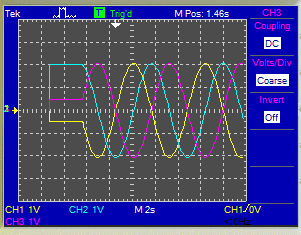
\includegraphics[width=1\textwidth]{Metodologia/SimulacionCondicionIniciales1.png}
    \captionof{figure}{Primera Simulación.}
    \label{fig}
\end{Figura}

Para la primera simulación se tomaron las condiciones iniciales $X_{0}=0.5m$ y $V_{0}=2m/s$, para esto se conectaron las respectivas fuentes de poder.
\\\\
El canal $1$ representa a la aceleración del oscilador armónico, el canal $2$ representa a la velocidad y el canal $3$ a la posición.


\begin{Figura}
    \centering
    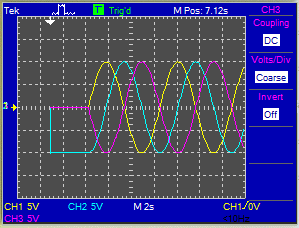
\includegraphics[width=1\textwidth]{Metodologia/SimulacionCondicionIniciales2.png}
    \captionof{figure}{Segunda Simulación.}
    \label{fig}
\end{Figura}

Para la segunda simulación se tomaron las condiciones iniciales $X_{0}=0m$ y $V_{0}=-10m/s$, para esto se conectaron las respectivas fuentes de poder.

\begin{Figura}
    \centering
    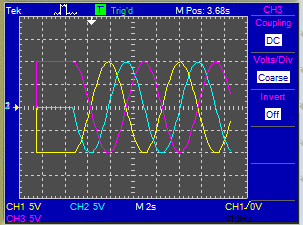
\includegraphics[width=1\textwidth]{Metodologia/SimulacionCondicionIniciales3.png}
    \captionof{figure}{Tercera Simulación.}
    \label{fig}
\end{Figura}

Para la tercera simulación se tomaron las condiciones iniciales $X_{0}=10m$ y $V_{0}=0m/s$, para esto se conectaron las respectivas fuentes de poder.

\section*{Conclusiones}

La simulación se llevó a cabo con éxito ya que cumple con la forma esperada dada por la teoría, las funciones obtenidas tienen la forma de la combinación de senos y cosenos.
\\\\
En las simulaciones podemos ver que cuando la aceleración es negativa la velocidad disminuye y cuando la velocidad es negativa la posición disminuye pero cuando la aceleración es positiva entonces la velocidad aumenta y cuando la velocidad es positiva la posición comienza a aumentar, esto concuerda y era lo esperado por la teoría de Osciladores Armónicos Simples.
  
\begin{thebibliography}{99}

\bibitem{1} Resnick, R., Halliday, D., & Krane, K. (2002a). Física. Vol. 1( 5ta Edición) (5.a ed.). Grupo Editorial Patria.

\bibitem{2} William Hart Hayt, Jack Ellsworth Kemmerly, Jamie D Phillips, and Steven M Durbin. 2019. Análisis de Circuitos En Ingeniería. Ciudad De México Mcgraw Hill Interamericana S.A. De C.V.

\bibitem{2} Floyd, Thomas L. Principios De Circuitos eléctricos (8a. Ed.). Naucalpan de Juárez: Pearson Educación, 2007.

\end{thebibliography}

%\section*{Apéndices}


\end{multicols}
\end{document}